\documentclass{beamer}
\usepackage{siunitx}
\usepackage{physics}
\usepackage[demo]{graphicx}
\usepackage{caption}
\usepackage{subcaption}
\usepackage[utf8]{inputenc}
\usepackage{multirow}

\usetheme{Warsaw}
\title{OPTIMIZATION}
\author{AAYUSH ARORA (EE17BTECH11003) }


\begin{document}

\maketitle 
\begin{frame}{QUESTION: 7.7 }
(Diet problem): A dietician wishes to mix two types of foods in such a way that vitamin contents of the mixture contain atleast 8 units of vitamin A and 10 units of vitamin C. Food ‘I’ contains 2 units/kg of vitamin A and 1 unit/kg of vitamin C. Food ‘II’ contains 1 unit/kg of vitamin A and 2 units/kg of
vitamin C. It costs Rs 50 per kg to purchase Food ‘I’ and Rs 70 per kg to purchase Food ‘II’. Formulate this problem as a linear programming problem to minimise the cost of such a mixture ?
\end{frame}





\begin{frame}{SOLUTION}
Let the mixture contains $x$ kg of food I and $y$ kg of food II.
\\
\begin{table}[]
\begin{tabular}{|l|l|l|l|}
\hline
\multirow{2}{*}{Resources} & \multicolumn{2}{l|}{Food} & \multirow{2}{*}{Requirement} \\ \cline{2-3}
                           & I           & II          &                              \\ \hline
Vitamin A                  & 2           & 1           & Atleast 8 Units              \\ \hline
Vitamin C                  & 1           & 2           & Atleast 10 Units             \\ \hline
Cost                       & 50          & 70          &                              \\ \hline
\end{tabular}
\end{table}
\end{frame}



\begin{frame}{}
GOAL: We need to minimize the cost of mixture.\\
Cost of FOOD I per kg = Rs 50 \\
Cost of FOOD II per kg = Rs 70 \\
 Minimize $ Z = 50x +70y$\\
 Subject to constraints:\\
 $2x+y>=8$\\
 $x+2y>=10$\\
 $x,y>=0$\\
 \end{frame}

\begin{frame}{}
  \begin{figure}

  \centering
  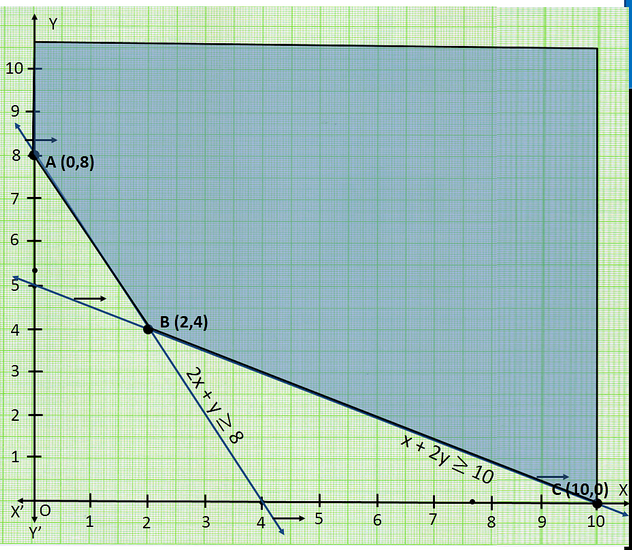
\includegraphics[width=1\linewidth]{fig.png}
  \end{figure}
\end{frame}



\begin{frame}{}
\begin{table}[]
\begin{tabular}{|l|l|l|l|}
\hline
Corner Point &  $Z=50x+70y$\\
\hline
(0,8)& 560\\
\hline
(2,4)& 380\\
\hline
(10,0)& 500\\
\hline
\end{tabular}
\end{table}
The smallest value of Z is 380 at the point (2,4). But the feasible region is unbounded therefore we draw the graph of the inequality:\\
$50x +70y<380$\\
to check whether the resulting open half has any point common with the feasible region but on checking it doesn't have any points in common. 


\end{frame}

\begin{frame}{}
Thus the minimum value of Z is 380 attained at (2,4). Hence optimal mixing strategy for the dietician would be to mix 2 Kg of Food I and 4 Kg of Food II.
\end{frame}


\section{Introduction}

\end{document}